\documentclass[../report.tex]{subfiles}


\begin{document}


\section{Introduction}
\label{introduction}

\subsection{What problem does the project focus on?}
\label{What problem does the project focus on?}


This project focuses on the problem of creating the best RL agent for a custom-made Reversi enviroment.
Reversi is a checkers-like piece-capturing board game where pieces are placed adjacent to existing opponent board pieces, capturing all opponent pieces between the new piece and the nearest ally piece.


This report focuses on our implementation of Reversi, which borrows many rules from the modern, Japanese version of reversi, Othello.
In particular, our implementation has a fixed starting state, and the game does not end when one player cannot make a legal move, the player simply passes their turn.
For the sake of this report, we will be exploring previous work on Reversi and Othello, as the similarities are greater then the differences for the sake of this use case.


Here is a simple example of a couple of moves in Reversi.
\begin{figure}[h]
    %\fbox{\rule[-.5cm]{0cm}{4cm} \rule[-.5cm]{10cm}{0cm}}
    \centering
    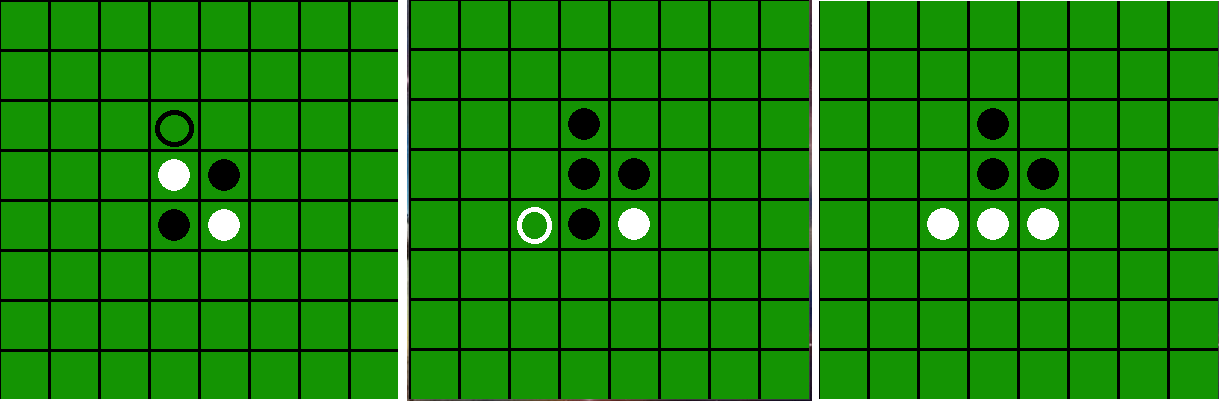
\includegraphics[width=10cm]{ReversiMoves}
    \caption{Two simple starting moves in Reversi}
\end{figure}
The game of reversi ends when neither player can make a legal move, which typically means the game board is filled.
Once the game has ended, the scoring is simple. The winner of Reversi is the player with the most game pieces on the board at the end of the game.


This problem is made complex by the $8\times8$ sized board which contains approximately $3^{64}$ possible states,
each with a set of actions $\geq0$.


With such a state and action space, tabular solutions are not practical, which makes different function approximation and Deep RL solutions attractive.
Since there are multiple methods to approach this problem, our project implements multiple algorithms and compares them against a baseline (Random) player and against each other.


In particular, this project explores Proximal Policy Optimization, Deep Q Network and its variants, and Deep SARSA


The agents are also trained differently in self-play or against random play to see which training method optimizes general performance.


The reward structure is built on the basis of having sparse rewards to allow the agents to discover the best methods of play.
We did not compare the sparse rewards model against different rewards models in this project.


Since in the case of reversi large sections of the game board can be captured in a few moves, the positioning of the player's pieces is more essential to winning than the number of pieces of each colour at different time steps.\
This is similar to the rewards structure of chess or checkers where the board's state can at times be conducive to a rapid victory for a colour, making intermediate rewards difficult to design without unintended consequences.


\subsection{Why should we care about this problem?}
\label{Why should we care about this problem?}


Since our problem is so similar to grid-based board games, our project may provide insights into the benefits and drawbacks of different RL agents in this space.


Our project uses ideas for different function approximation algorithms with similar board games from other projects,
which means that some of the insights gleaned in the design of RL algorithms for solving board games may be generalized to all board games, and could even be useful in solving tile-based strategy games.


In addition, the selection of multiple function approximation algorithms allows us to learn much more about the optimal learning methods, hyperparameters, and learning times for these different algorithms.
Specifically, we can learn how algorithms taught with self-play interact with eachother or with the random agent and evaluate tailored learning methods for each algorithm.


In summary, there is a significant amount of specific knowledge in the development of this project that provides insights about RL in Reversi
and also function approximation and Deep RL in comparison to eachother.
In addition, the insight gleaned in this project has the possibility of expanding beyond this specific problem into general problems in board and strategy games.


\subsection{The goal of this report}
\label{The goal of this report}


The goal of this report is firstly to detail to the reader the existing knowledge on Reversi/Othello in the RL space.


To study multiple approaches to Reversi as a RL problem, and to compare these approaches.


Finally, this report aims to use the results of the empirical studies done on the chosen RL methods to gain insights into the methods,
the implementation of the methods, Reversi as an RL problem, and RL in board and strategy games as a whole.


\subsection{The sections of this report}
\label{The sections of this report}


This report is made up of 4 different sections.
Section 1 has been an introduction to Reversi and our project and answers what problem the project focuses on and why that problem is significant.


Section 2 reviews previous work on Reversi/Othello, details the RL approaches in our project, and justifies the choices made in the algorithms used via experiments or reasoning.


Section 3 Outlines Empirical studies conducted in this report, compares the various approaches using experiments, and discusses the different aspects of the results of the experiments.


Section 4 Concludes the report by answering what we have learned from the project, and how we would improve methodology given more time and resources.


\end{document}